\chapter{Photons and Phonons}\label{ch:b3:photons-phonons}

Quantum theory was born in this chapter's subject. In 1900 the
spectrum of glowing bodies refused to obey classical physics ---
worse, classical physics predicted \emph{infinite} energy at short
wavelengths, the ``ultraviolet catastrophe'' --- and Planck's
desperate remedy, energy in packets of $h\nu$, turned out to be the
century's master key. With the machinery now assembled --- mode
counting from \cref{ch:b3:schrodinger-three-dimensions}, oscillator
thermodynamics from \cref{ch:b3:canonical-ensemble} --- \omterm{thm:b3:photons-phonons:planck}{Planck's law}
takes half a page: a gas of photons, one Bose-occupied oscillator
per cavity mode. The same half page, with sound in place of light,
is Debye's theory of solids and the $T^3$ heat capacity Einstein's
model missed. And filling every cubic centimetre of the universe is
the subject's masterpiece: the 2.725-kelvin cosmic microwave
background, the most perfect blackbody ever measured --- the
thermal radiation of the young universe itself, still arriving.

\section{Planck's law, derived}

\begin{theorem}[The blackbody spectrum]\label{thm:b3:photons-phonons:planck}
\index{Planck's law}\index{blackbody radiation}
A cavity at temperature $T$ supports electromagnetic modes ---
standing waves counted exactly as in
\cref{prop:b3:schrodinger-three-dimensions:counting}, twice for
polarisation:
\[
g(\nu)\,\dd\nu = \frac{8\pi V}{c^3}\,\nu^2\,\dd\nu .
\]
Each mode is a quantum oscillator holding, at equilibrium,
$\bar n = 1/(\eu^{h\nu/k_{\text{B}}T} - 1)$ photons
(\cref{exo:b3:canonical-ensemble:5}; equivalently, bosons at $\mu =
0$). The energy per volume and frequency is therefore
\[
u(\nu, T) = \frac{8\pi h\nu^3}{c^3}\,
\frac{1}{\eu^{h\nu/k_{\text{B}}T} - 1} :
\]
\emph{\omterm{thm:b3:photons-phonons:planck}{Planck's law}} (1900). Its consequences, all as measured:
the peak at $\lambda_{\max}T = \qty{2898}{\micro m.K}$ (Wien's
displacement law of the Year 2 volume, now derived); the total flux
from a black surface $\Phi = \sigma T^4$ with
\[
\sigma = \frac{2\pi^5k_{\text{B}}^4}{15h^3c^2}
 = \qty{5.67e-8}{W.m^{-2}.K^{-4}}
\]
(Stefan--Boltzmann, its constant now built from $h$, $c$,
$k_{\text{B}}$); and the photon density $n_\gamma \approx
\num{2.03e7}\,(T/\unit{K})^3$ per cubic metre.
\end{theorem}

\begin{proof}[Partial proof]
Multiply the mode count by $h\nu\,\bar n$. The total energy
integral, with $x = h\nu/k_{\text{B}}T$ and $\int_0^\infty
x^3\dd x/(\eu^x - 1) = \pi^4/15$ (admitted), gives $u_{\text{tot}}
= aT^4$ and, with the standard flux factor $c/4$, the stated
$\sigma$. Wien's law is the maximisation of
\cref{exo:b3:photons-phonons:1}. At low frequency ($h\nu \ll
k_{\text{B}}T$) each mode carries $k_{\text{B}}T$ ---
Rayleigh--Jeans, correct for radio, catastrophic if extended to all
$\nu$: Planck's cutoff is equipartition's licence
(\cref{thm:b3:canonical-ensemble:equipartition}) being revoked
mode by mode.
\end{proof}

\begin{omfigure}
\begin{tikzpicture}
  \begin{axis}[omaxis, axis x line=bottom, axis y line=left,
    width=11.4cm, height=6.0cm, xmin=0, xmax=4.4, ymin=0, ymax=1.5,
    xlabel={$\nu$ (units of $10^{14}$ Hz)}, ylabel={$u(\nu)$ (scaled)},
    xlabel style={at={(axis description cs:0.5,-0.09)}, anchor=north},
    xtick={1,2,3,4}, ytick=\empty, clip=false,
    legend style={font=\scriptsize, at={(0.97,0.93)}, anchor=north east,
      draw=none, fill=none}]
    \addplot[omDef, very thick, domain=0.01:4.4, samples=200]
      {1.42*x^3/(exp(x/1.208)-1)/8.3};
    \addlegendentry{$T = \qty{5800}{K}$ (the Sun)}
    \addplot[omThm, thick, domain=0.01:4.4, samples=200]
      {1.42*x^3/(exp(x/0.833)-1)/2.72};
    \addlegendentry{$T = \qty{4000}{K}$}
    \addplot[omExo, thick, domain=0.01:4.4, samples=200]
      {1.42*x^3/(exp(x/0.625)-1)/1.15};
    \addlegendentry{$T = \qty{3000}{K}$}
    \addplot[gray, dashed, domain=0.01:1.9, samples=100]
      {1.42*x^2*1.208/8.3};
    \node[gray, font=\scriptsize, anchor=west, rotate=48] at (axis cs:1.28,0.62)
      {Rayleigh--Jeans};
  \end{axis}
\end{tikzpicture}

{\small Planck spectra at three temperatures (each scaled to
comparable height: the true areas grow as $T^4$). The classical
Rayleigh--Jeans line follows the low-frequency flank and then
soars toward the ultraviolet catastrophe; Planck's $h\nu$ toll
closes the high-frequency modes and bends the curve down.}
\end{omfigure}

\begin{example}[Three thermometers]\label{ex:b3:photons-phonons:thermometers}
The Sun ($T = \qty{5800}{K}$): peak at \qty{0.50}{\micro m} ---
our eyes evolved onto its maximum. A body at \qty{310}{K}: peak
near \qty{9.4}{\micro m}, radiating $\sigma T^4 \approx
\qty{520}{W/m^2}$ from every square metre of skin (mercifully, the
room radiates back;
\cref{exo:b3:photons-phonons:2}). The universe ($T =
\qty{2.725}{K}$): peak near \qty{1.9}{mm} in frequency form
(\qty{160}{GHz}), $411$ photons per cubic centimetre ---
the cosmic microwave background, this chapter's grand example
(\cref{pb:b3:photons-phonons:1}).
\end{example}

\begin{proposition}[Thermodynamics of light]\label{prop:b3:photons-phonons:thermo}
\index{radiation pressure!thermal}
The photon gas has energy density $u = aT^4$ ($a =
4\sigma/c$), pressure
\[
P = \frac u3 ,
\]
entropy density $\tfrac43 aT^3$, and photon number $\propto T^3$.
Consequences: an adiabatically expanding radiation-filled box
cools as $T \propto 1/L$ --- the expanding universe's photons
cooled from $3000$ K to today's $2.725$ K by a stretch factor
$\approx1100$ while \emph{keeping} a perfect Planck spectrum; and
in massive stars the $T^4$ growth lets radiation pressure rival
gas pressure, setting an upper limit to stellar masses
(\cref{ch:b3:astrophysics}).
\end{proposition}

\begin{proof}[Partial proof]
$P = u/3$: an isotropic gas of particles at speed $c$ delivers
one-third of its energy density as pressure (the factor $\langle
\cos^2\theta\rangle = 1/3$, as in the kinetic theory of the Year 1
volume). Entropy from $\dd U = T\dd S - P\dd V$ applied to $U =
aT^4V$. Adiabatic: $S \propto T^3V$ constant gives $T \propto
V^{-1/3}$.
\end{proof}

\section{Phonons: Debye's completion}

\begin{theorem}[The Debye model]\label{thm:b3:photons-phonons:debye}
\index{Debye model}\index{phonon}
A crystal's vibrations are \omterm{prop:b3:continuum-elasticity:waves}{elastic waves} quantised exactly like
light: \emph{phonons}, three polarisations at sound speed
$c_{\text{s}}$, counted like photons but with the total capped at
$3N$ modes --- the cap defining the \emph{Debye temperature}
\[
k_{\text{B}}\theta_{\text{D}} = \hbar c_{\text{s}}
(6\pi^2n)^{1/3} .
\]
The heat capacity interpolates between the two classic laws:
\[
C \to 3Nk_{\text{B}} \;(T \gg \theta_{\text{D}})
\qquad\text{(Dulong--Petit)} ,
\qquad
C \to \frac{12\pi^4}{5}\,Nk_{\text{B}}
\Big(\frac{T}{\theta_{\text{D}}}\Big)^3
\;(T \ll \theta_{\text{D}}) :
\]
the $T^3$ law that low-temperature calorimetry demanded and
Einstein's single frequency could not give
(\cref{exo:b3:canonical-ensemble:6}). The reason is the same as
for light: however cold the crystal, arbitrarily cheap
long-wavelength sound quanta exist, and their photon-like counting
gives the photon-like $T^3$.
\end{theorem}

\begin{proof}[Partial proof]
Repeat the photon computation with $c \to c_{\text{s}}$, three
polarisations, and the mode total $\int g\,\dd\nu = 3N$ fixing the
cutoff. At $T \ll \theta_{\text{D}}$ the cutoff is invisible and
the $T^4$ energy integral gives $C \propto T^3$; at high $T$ every
one of the $3N$ modes carries $k_{\text{B}}T$. The full
interpolation integral is admitted.
\end{proof}

\begin{omfigure}
\begin{tikzpicture}
  \begin{axis}[omaxis, axis x line=bottom, axis y line=left,
    width=11.0cm, height=5.6cm, xmin=0, xmax=1.5, ymin=0, ymax=1.15,
    xlabel={$T/\theta_{\text{D}}$}, ylabel={$C/3Nk_{\text{B}}$},
    xlabel style={at={(axis description cs:0.5,-0.1)}, anchor=north},
    xtick={0.5,1,1.5}, ytick={0.5,1}, clip=false,
    legend style={font=\scriptsize, at={(0.95,0.42)}, anchor=north east,
      draw=none, fill=none}]
    \addplot[gray, dashed, domain=0:1.5, forget plot] {1};
    \addplot[omDef, very thick, domain=0.02:1.5, samples=200]
      {1/(1+0.01283/(x*x*x))};
    \addlegendentry{Debye}
    \addplot[omExo, thick, dashed, domain=0.02:1.5, samples=200]
      {(0.75/x)^2*exp(-0.75/x)/(1-exp(-0.75/x))^2};
    \addlegendentry{Einstein}
    \node[omDef, font=\scriptsize, anchor=west] at (axis cs:0.2,0.28)
      {$\propto T^3$};
    \draw[->, omDef] (axis cs:0.2,0.24) -- (axis cs:0.13,0.13);
  \end{axis}
\end{tikzpicture}

{\small Heat capacity of a crystal: both models reach
Dulong--Petit, but at low temperature Einstein's single-frequency
curve dies exponentially while Debye's cheap long-wavelength
phonons sustain the measured $T^3$ --- the low-$T$ region is pure
``photon physics'' with sound.}
\end{omfigure}

\begin{example}[Phonons are real particles]\label{ex:b3:photons-phonons:phonon-real}
Phonons scatter neutrons and X-rays with energy and (crystal)
momentum conservation --- the measured dispersion curves
$\omega(\vect k)$ of \cref{ch:b3:crystalline-solids} are their
spectroscopy. They carry heat: an insulator's thermal conductivity
is a phonon gas's $\kappa = \tfrac13 Cc_{\text{s}}\ell$, and
diamond --- stiff, light, pure --- outconducts copper fivefold at
room temperature by phonons alone
(\cref{exo:b3:photons-phonons:12}). And they die out at low
temperature as $T^3$, which is why cryogenic engineers speak of
crystals going ``acoustically silent''.
\end{example}

\begin{method}[Radiation-gas craft]\label{met:b3:photons-phonons:method}
(1) Count modes ($\propto\nu^2$ per polarisation in 3D); occupy
with $1/(\eu^{\beta h\nu} - 1)$; integrate --- expect $T^4$
energies and $T^3$ counts and capacities. (2) Peaks via Wien;
totals via Stefan; per-mode classical $k_{\text{B}}T$ only below
$h\nu \sim k_{\text{B}}T$. (3) For solids, cap the modes at $3N$
($\theta_{\text{D}}$); Einstein's form for optical-branch modes,
Debye's for acoustic. (4) Adiabatic radiation: $T \propto
V^{-1/3}$. (5) Check the two constants of the trade: $\lambda_{
\max}T = \qty{2898}{\micro m.K}$ and $\sigma =
\qty{5.67e-8}{W/m^2K^4}$.
\end{method}

\begin{omfigure}
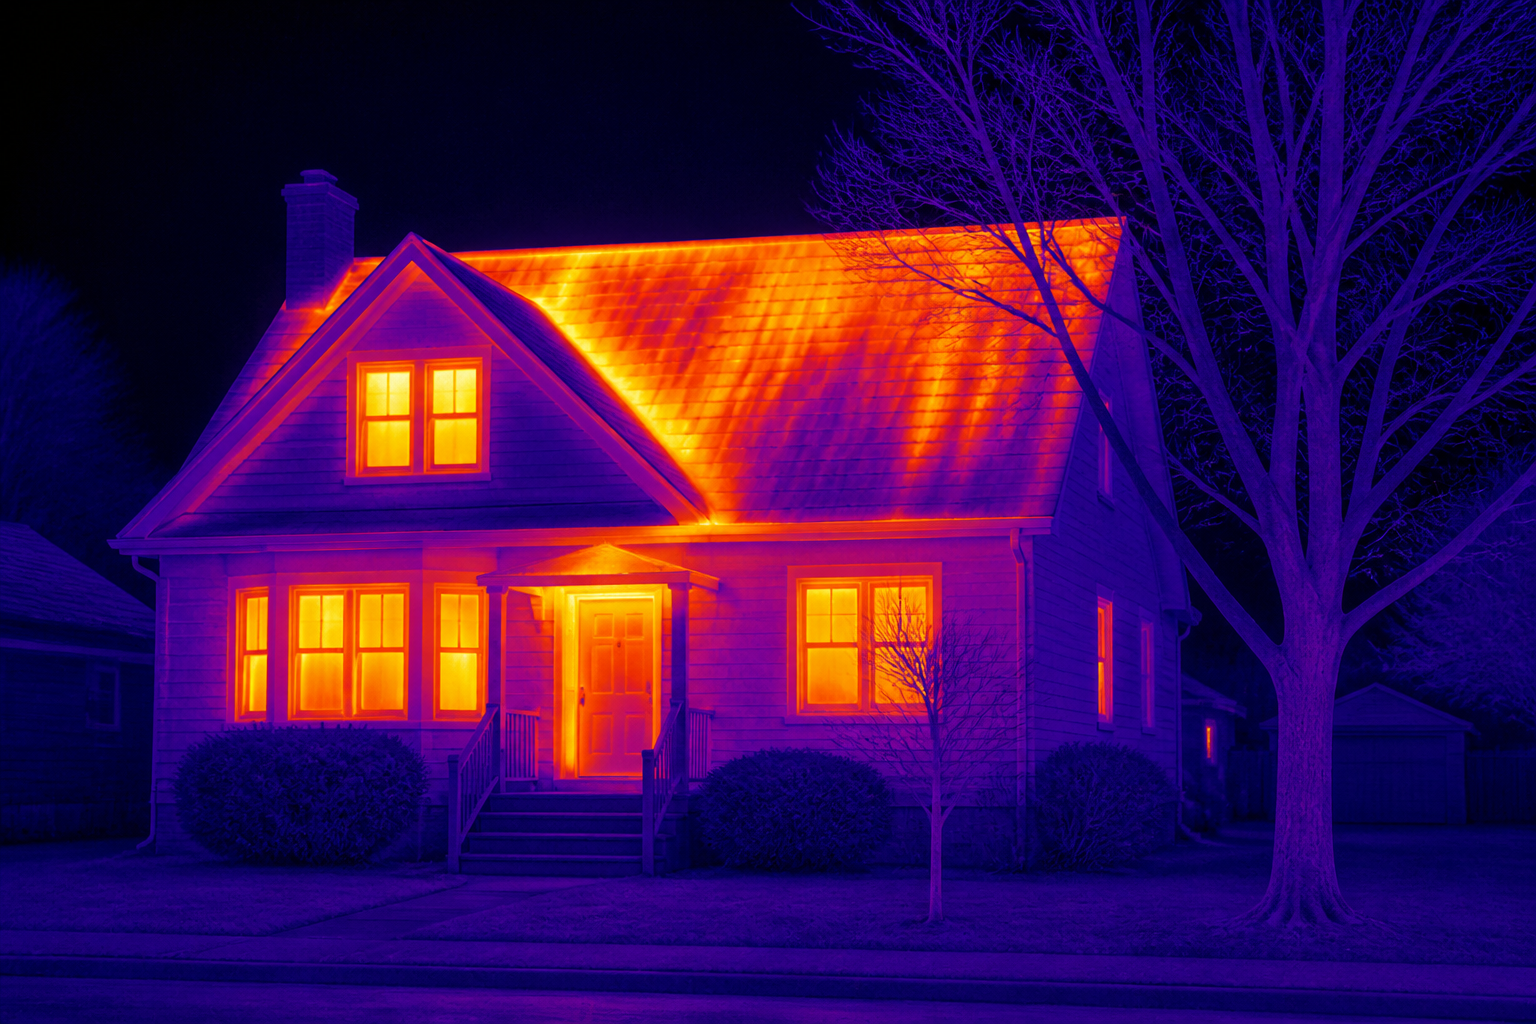
\includegraphics[width=0.58\linewidth]{images/book5/ai/b5-09-thermal-house.png}

{\small A house through a thermal camera: every surface radiates its Planck spectrum, and the camera reads temperature straight off the infrared --- Stefan, Boltzmann and Wien auditing the heating bill.}
\end{omfigure}

\section{Exercises}

\begin{exercise}[$\star$]\label{exo:b3:photons-phonons:1}
(a) From \omterm{thm:b3:photons-phonons:planck}{Planck's law} in wavelength form, show the peak obeys
$\lambda_{\max}T = $ const (the transcendental equation may be
cited: $x = 4.965$). (b) Compute the peak wavelengths for the
Sun, a \qty{2700}{K} filament, a \qty{310}{K} body and the
\qty{2.725}{K} sky. (c) Which of the four does the human eye
sample well, and what fraction of a filament's output is visible
(estimate: small)? (d) Why are ``infrared cameras'' the right
tool for people and buildings?
\end{exercise}

\begin{exercise}[$\star$]\label{exo:b3:photons-phonons:2}
Radiative budgets. (a) A person ($\qty{1.7}{m^2}$, skin
\qty{306}{K}) in a \qty{293}{K} room: net radiated power
$\sigma A(T_1^4 - T_2^4)$. (b) Compare with the body's
\qty{100}{W} metabolism: why do we tolerate it (clothing, and the
room radiating back)? (c) The Earth absorbs sunlight over $\pi
R^2$ and radiates over $4\pi R^2$: derive $T_{\text{eff}}
= [(1-A)\,\Phi_\odot/4\sigma]^{1/4}$ with $\Phi_\odot =
\qty{1361}{W/m^2}$, albedo $A = 0.30$, and evaluate. (d) The
measured surface average is \qty{288}{K}: name the mechanism of
the \qty{33}{K} difference
(\cref{pb:b3:harmonic-oscillator:1}).
\end{exercise}

\begin{exercise}[$\star$]\label{exo:b3:photons-phonons:3}
Counting photons. (a) With $n_\gamma = \num{2.03e7}\,T^3$ per
cubic metre: the photon density of the \qty{2.725}{K} background.
(b) Sunlight at Earth: from $\Phi_\odot$ and a mean photon energy
$\approx 2.7\,k_{\text{B}}T_\odot \approx \qty{1.35}{eV}$,
compute the photon flux per square metre per second. (c) A
\qty{60}{W} incandescent bulb (5\% visible): visible photons per
second. (d) Why is ``photon counting'' routine for astronomers
but absurd for heaters?
\end{exercise}

\begin{exercise}[$\star$]\label{exo:b3:photons-phonons:4}
The catastrophe and its tail. (a) Show classical equipartition
($k_{\text{B}}T$ per mode) gives $u(\nu) =
8\pi\nu^2k_{\text{B}}T/c^3$, divergent when integrated. (b) Where
does \omterm{thm:b3:photons-phonons:planck}{Planck's law} reduce to it? (c) Radio astronomers measure the
CMB at \qty{1.4}{GHz}: check $h\nu/k_{\text{B}}T \ll 1$ there and
justify their ``antenna temperature'' habit of quoting intensities
in kelvin. (d) At the CMB's \qty{160}{GHz} peak, evaluate
$h\nu/k_{\text{B}}T$: is the peak classical?
\end{exercise}

\begin{exercise}[$\star\star$]\label{exo:b3:photons-phonons:5}
Radiation pressure. (a) Derive $P = u/3$ from isotropy (or accept
the kinetic factor) and evaluate the pressure of sunlight at
Earth's orbit; compare with atmospheric pressure. (b) Inside the
Sun ($T \approx \qty{1.5e7}{K}$): compute $P_{\text{rad}} =
aT^4/3$ and compare with the gas pressure $\sim\qty{2e16}{Pa}$.
(c) Radiation pressure grows as $T^4$, gas pressure as $T$: show
why sufficiently massive (hence hotter) stars become
radiation-dominated and unstable --- the Eddington ceiling near
$\sim100\,M_\odot$. (d) Lasers: a \qty{1}{kW} beam focused to
push --- what force? Why do ``tractor beams'' stay in movies while
optical \emph{tweezers} (gradients, piconewtons) are real tools?
\end{exercise}

\begin{exercise}[$\star\star$]\label{exo:b3:photons-phonons:6}
The universe's stretch. The CMB was emitted at recombination
($T \approx \qty{3000}{K}$, \cref{exo:b3:grand-canonical:12}
territory) and arrives at \qty{2.725}{K}. (a) From $T \propto
1/a$, the stretch factor of all lengths since emission. (b) Show
a Planck spectrum stays Planck under uniform stretching of every
wavelength (what happens to $T$?). (c) The emitted peak (visible
orange light!) arrives where? (d) Why is the sky therefore dark
to the eye yet blazing to a microwave receiver?
\end{exercise}

\begin{exercise}[$\star\star$]\label{exo:b3:photons-phonons:7}
Debye temperatures from sound. (a) Evaluate $\theta_{\text{D}} =
\hbar c_{\text{s}}(6\pi^2n)^{1/3}/k_{\text{B}}$ for copper
($c_{\text{s}} \approx \qty{3800}{m/s}$, $n =
\qty{8.5e28}{m^{-3}}$) and compare with the calorimetric
\qty{343}{K}. (b) Diamond: $c_{\text{s}} \approx
\qty{13000}{m/s}$, $n = \qty{1.76e29}{m^{-3}}$: compute and
compare with $\approx\qty{2200}{K}$. (c) Lead: soft and heavy ---
explain its $\theta_{\text{D}} \approx \qty{90}{K}$ in one
sentence. (d) State the rule connecting a solid's stiffness,
atomic mass and its quantum-freezing temperature.
\end{exercise}

\begin{exercise}[$\star\star$]\label{exo:b3:photons-phonons:8}
Copper at one kelvin. (a) Using $C = \gamma T + \beta T^3$ with
$\gamma$ from \cref{ex:b3:quantum-statistics:heat} and the Debye
$T^3$ coefficient for $\theta_{\text{D}} = \qty{343}{K}$: compute
both terms per mole at \qty{1}{K}. (b) Which wins, and by how
much? (c) At what temperature do they cross? (d) Why is this
regime the calorimetrist's window onto the electronic \omterm{prop:b3:schrodinger-three-dimensions:counting}{density of
states}?
\end{exercise}

\begin{exercise}[$\star\star$]\label{exo:b3:photons-phonons:9}
One-layer greenhouse. Let the surface (temperature $T_s$) sit
under one thin atmospheric layer (temperature $T_a$) transparent
to sunlight but opaque to thermal infrared. (a) Write energy
balance for the layer (absorbs $\sigma T_s^4$, radiates
$2\sigma T_a^4$) and for the surface (absorbs sunlight $S$ plus
$\sigma T_a^4$). (b) Show $T_s = 2^{1/4}\,T_{\text{eff}}$ where
$\sigma T_{\text{eff}}^4 = S$. (c) With $T_{\text{eff}} =
\qty{255}{K}$: evaluate $T_s$ and compare with \qty{288}{K}
(the real atmosphere is a partial, multi-layer blanket). (d)
Connect to \cref{pb:b3:harmonic-oscillator:1}: which molecular
physics makes the layer opaque in the infrared yet transparent in
the visible?
\end{exercise}

\begin{exercise}[$\star\star\star$]\label{exo:b3:photons-phonons:10}
Stefan's constant from scratch. (a) Assemble $u_{\text{tot}} =
\int u(\nu)\dd\nu$ with $x = h\nu/k_{\text{B}}T$ and the given
$\pi^4/15$, obtaining $u = aT^4$ with $a =
8\pi^5k_{\text{B}}^4/15h^3c^3$. (b) The flux from a black
surface is $c\,u/4$ (accept the geometric quarter): form
$\sigma$ and evaluate it numerically from $h$, $c$,
$k_{\text{B}}$. (c) Compare with \qty{5.67e-8}{W.m^{-2}.K^{-4}}.
(d) Historical inversion: Planck fitted his law to spectra and
extracted \emph{both} $h$ and $k_{\text{B}}$ (hence Avogadro's
number) in 1900 --- state why the blackbody curve pins two
constants at once.
\end{exercise}

\begin{exercise}[$\star\star\star$]\label{exo:b3:photons-phonons:11}
Einstein's A and B (1917). Two-level atoms (energies $0,
h\nu_0$; populations $N_1, N_2$) sit in radiation of spectral
density $u(\nu_0)$. Absorption rate: $B_{12}uN_1$; stimulated
emission: $B_{21}uN_2$; spontaneous: $AN_2$. (a) Write the
equilibrium balance. (b) Demand that the Boltzmann ratio
$N_2/N_1 = \eu^{-h\nu_0/k_{\text{B}}T}$ and Planck's $u$ hold
simultaneously for \emph{all} $T$: derive $B_{12} = B_{21}$ and
\[
\frac{A}{B} = \frac{8\pi h\nu_0^3}{c^3} .
\]
(c) Interpret: why does thermal equilibrium \emph{force}
spontaneous emission to exist, and fix its rate from the
stimulated one? (d) The $\nu^3$: connect to
\cref{exo:b3:perturbation-theory:8}'s lifetimes and to why lasing
is hard at X-ray frequencies.
\end{exercise}

\begin{exercise}[$\star\star\star$]\label{exo:b3:photons-phonons:12}
Diamond, the phonon superhighway. Thermal conductivity of an
insulator: $\kappa = \tfrac13 C_v c_{\text{s}}\ell$ per volume,
with $\ell$ the phonon mean free path. (a) For diamond at
\qty{300}{K} ($C_v \approx \qty{1.8e6}{J.m^{-3}K^{-1}}$, i.e.\
partially frozen; $c_{\text{s}} = \qty{13000}{m/s}$; $\ell
\approx \qty{0.3}{\micro m}$): compute $\kappa$ and compare with
copper's \qty{400}{W/(m.K)}. (b) Why is $\ell$ so long in diamond
(stiff, light, isotopically clean --- what scatters phonons?).
(c) Isotopically purified diamond nearly doubles $\kappa$: what
does that reveal about phonon scattering by isotopic mass
disorder? (d) Two uses: heat spreaders in electronics; and why a
diamond feels cold to the lip --- explain the sensation.
\end{exercise}

\begin{omfigure}
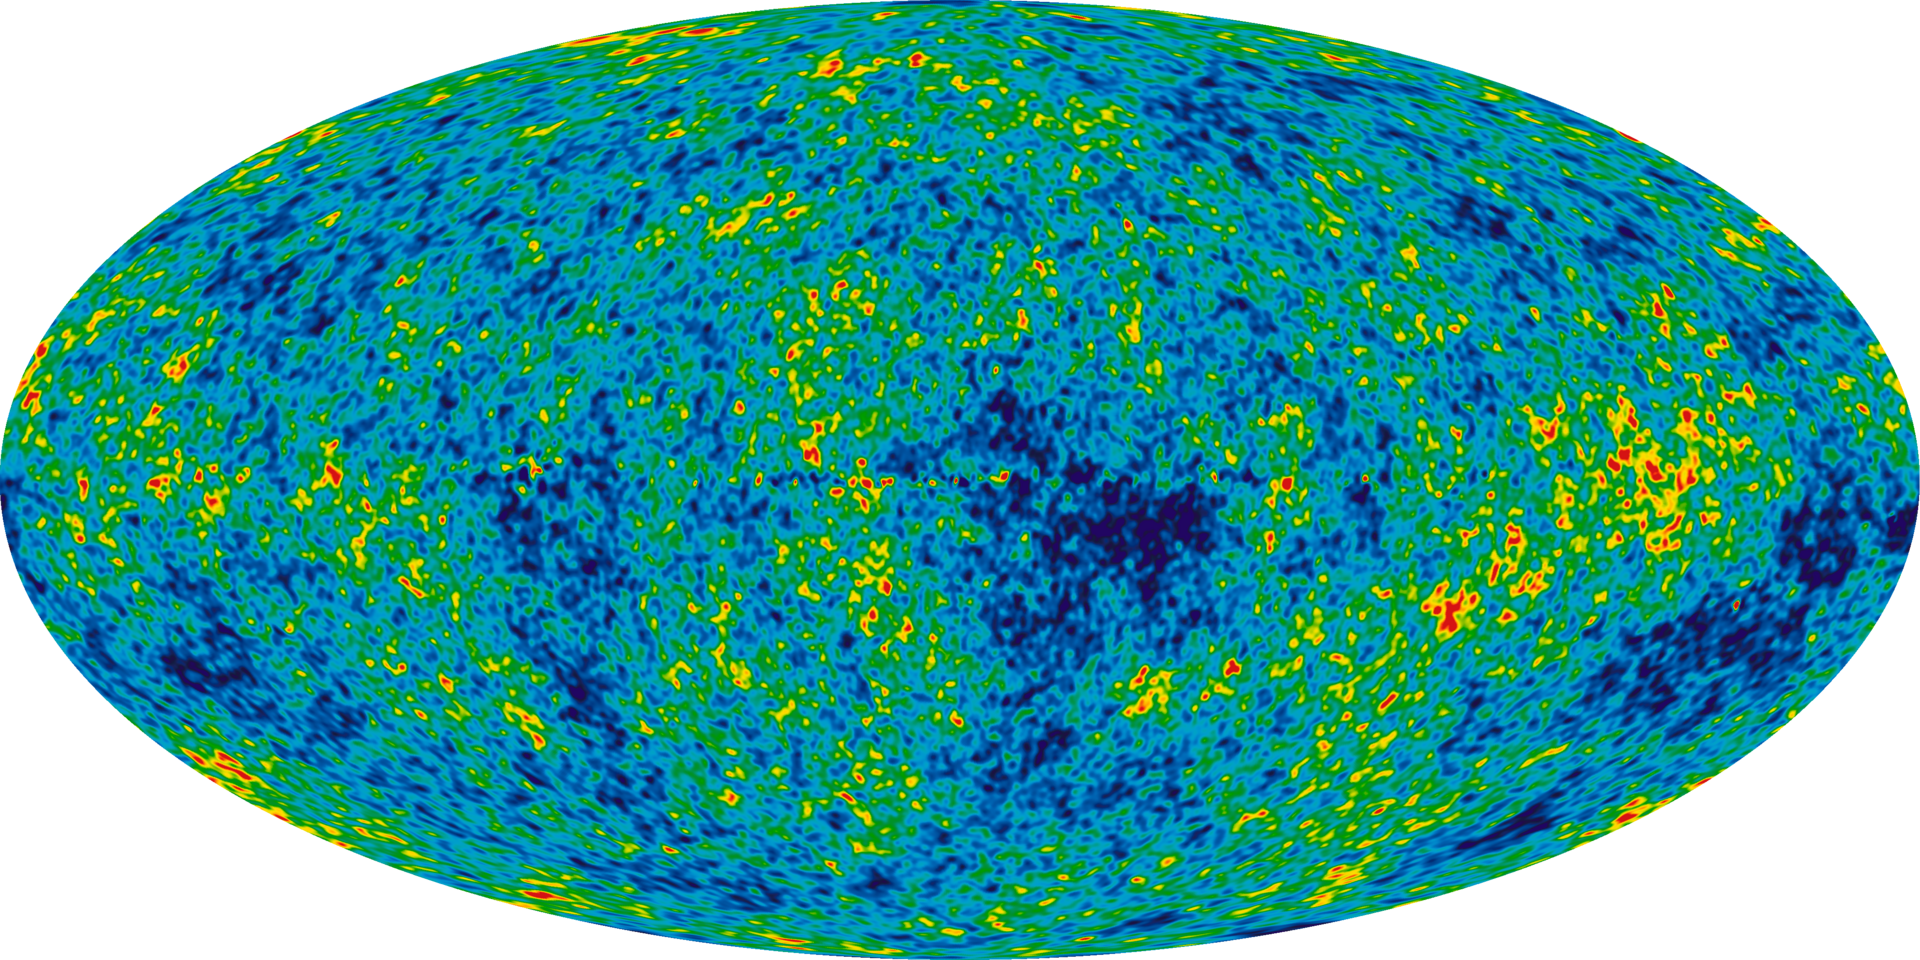
\includegraphics[width=0.62\linewidth]{images/book5/photo-cmb-wmap.png}

{\small The whole sky in microwaves (NASA/WMAP, public domain): the cosmic background's \qty{2.7}{K} Planck radiation, mapped. The mottling is one part in $10^5$ --- the seeds of galaxies, printed on this chapter's blackbody.}
\end{omfigure}

\section{Problem: The oldest light}

\begin{problem}[{Weekend problem --- reading the cosmic microwave
background}]\label{pb:b3:photons-phonons:1}
Point any millimetre-wave receiver at any patch of sky and it
reports the same signal: a Planck spectrum at $T =
\qty{2.72548(57)}{K}$, smoother than any furnace mankind has
built. It is the flash of the universe's recombination
(\cref{exo:b3:grand-canonical:12}), stretched eleven-hundred-fold,
and it carries the census of the cosmos. Data: $T_0 =
\qty{2.725}{K}$; $n_\gamma = \num{2.03e7}\,T^3\,\unit{m^{-3}}$;
$u = aT^4$, $a = \qty{7.56e-16}{J.m^{-3}.K^{-4}}$; baryon density
today $n_{\text{b}} \approx \qty{0.25}{m^{-3}}$; critical density
$\rho_{\text{c}} \approx \qty{8.6e-27}{kg/m^3}$.

\medskip\noindent\textbf{Part I --- The spectrum.}
\begin{enumerate}
  \item Compute the CMB's peak (Wien) wavelength and its photon
        density per cubic centimetre.
  \item Compute its energy density, in $\unit{J/m^3}$ and in
        $\unit{eV/cm^3}$, and its mass-equivalent fraction of the
        critical density.
  \item COBE's spectrum (1990) matched Planck to a few parts in
        $10^4$ --- the audience applauded the graph. Why is a
        \emph{perfect thermal} spectrum from empty sky so hard to
        explain by anything except a hot dense past?
  \item At emission the same photons formed a \qty{3000}{K}
        blackbody: check the stretch factor $1 + z =
        T_{\text{then}}/T_0$.
  \item Why did the universe become transparent at just that
        temperature (recall which equilibrium of
        \cref{ch:b3:grand-canonical} switched off)?
  \item The night sky is dark (Olbers' paradox of the old
        astronomy): in what precise sense is it actually
        \emph{bright} --- at what wavelength and temperature?
\end{enumerate}

\medskip\noindent\textbf{Part II --- The census.}
\begin{enumerate}[resume]
  \item Compute the photon-to-baryon ratio $\eta^{-1} =
        n_\gamma/n_{\text{b}}$.
  \item That number --- around two billion photons per proton ---
        is one of cosmology's fundamental data: state what it
        measures about the matter--antimatter asymmetry (recall
        \cref{exo:b3:grand-canonical:12}: the photons are mostly
        annihilation products).
  \item Compare the CMB's energy density with starlight's
        ($\sim\qty{2e-15}{J/m^3}$ averaged over the universe):
        which light dominates the cosmos?
  \item The CMB outweighs, in photons, everything stars have ever
        shone: why does this make the early universe
        ``radiation-dominated'', and what took over later (the
        $T^4$ versus $T^3$ scalings against matter's $a^{-3}$)?
  \item Estimate the epoch of matter--radiation equality: with
        radiation density scaling as $(1+z)^4$ and matter as
        $(1+z)^3$, and today's ratio
        $u_{\text{rad}}/\rho_{\text{m}}c^2 \approx 1/3400$, find
        $z_{\text{eq}}$.
  \item Neutrinos decoupled earlier and cooled slightly more
        (they missed the $e^+e^-$ annihilation reheat of
        \cref{exo:b3:grand-canonical:12}): the predicted
        $T_\nu = (4/11)^{1/3}T_\gamma$ --- evaluate it, and
        marvel at a prediction of a \qty{1.95}{K} neutrino sea
        nobody has yet directly detected.
\end{enumerate}

\medskip\noindent\textbf{Part III --- The anisotropies.}
\begin{enumerate}[resume]
  \item The CMB is \qty{3.4}{mK} hotter in one direction and
        cooler opposite: interpret via the Doppler physics of
        \cref{ch:b3:relativistic-kinematics} and extract our
        velocity ($\Delta T/T = v/c$).
  \item After removing that dipole, ripples of $\Delta T/T \sim
        \num{e-5}$ remain (COBE 1992, then WMAP, Planck): what do
        they map at $z = 1100$?
  \item Those $10^{-5}$ density seeds grew into galaxies: why
        does gravity amplify overdensities (which instability),
        and why did growth need matter--radiation equality to
        begin in earnest?
  \item The strongest ripple size (about one degree on the sky)
        is an acoustic wavelength --- sound in the
        photon--baryon plasma (this chapter's gas plus
        \cref{ch:b3:continuum-elasticity}'s waves!): what sets
        its scale (the distance sound travels before
        recombination)?
  \item Measuring that angle against the known physical scale
        triangulates the geometry of the universe: state the
        result (flat, to percent precision).
  \item The \qty{2.7}{K} monopole, the \qty{3}{mK} dipole, the
        \qty{e-5} ripples: rank what each has taught (a hot past;
        our motion; the seeds and geometry of everything).
\end{enumerate}

\medskip\noindent\textbf{Part IV --- The heirloom.}
\begin{enumerate}[resume]
  \item Penzias and Wilson found the signal in 1965 as
        irremovable antenna noise (after evicting the pigeons):
        why was an \emph{isotropic}, season-independent excess at
        \qty{3}{K} inexplicable as any local or galactic source?
  \item About $1\%$ of an untuned analogue television's static
        was this signal: reflect in one sentence.
  \item The CMB passes through galaxy clusters and gets slightly
        kicked to higher frequency by hot electrons (the
        Sunyaev--Zel'dovich effect): why does this make clusters
        visible as \emph{shadows} at low frequency, and what is
        such a shadow's special virtue (independent of
        distance)?
  \item Today's frontier hunts the CMB's polarisation for the
        imprint of primordial gravitational waves: which chapters
        of this book would that discovery marry
        (\cref{ch:b3:covariant-electromagnetism}'s polarisation,
        gravity's waves)?
  \item Compute the flux of CMB photons through your body
        ($n_\gamma c/4$ per unit area, body \omterm{def:b3:scattering-theory:cross-section}{cross-section}
        $\sim\qty{0.5}{m^2}$): how many relics of the Big Bang
        cross you per second?
  \item The CMB singles out a rest frame (the one where the
        dipole vanishes): explain why this does \emph{not}
        contradict relativity --- what kind of frame is preferred
        by the matter content rather than by the laws?
  \item Summarise the named result: a $2.725$-kelvin Planck
        curve filling the sky --- $411$ photons per cubic
        centimetre, two billion per baryon, peak at
        \qty{160}{GHz} --- is the thermal receipt of the hot
        beginning: statistical physics as cosmology's foundation
        stone.
\end{enumerate}
\end{problem}
